\chapter{Application features and manual}

\section{Add new tabs}

After starting the application the window looks like this: \\
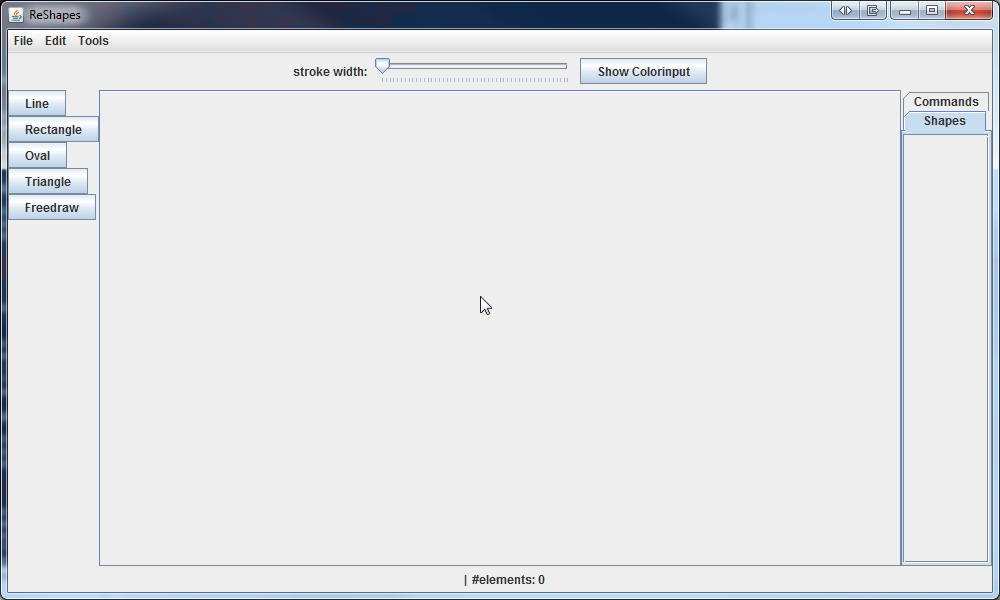
\includegraphics[width=1\textwidth]{img/startup_window} \\

To start drawing you have to add tab with \textbf{File $\rightarrow$ New Tab} \\
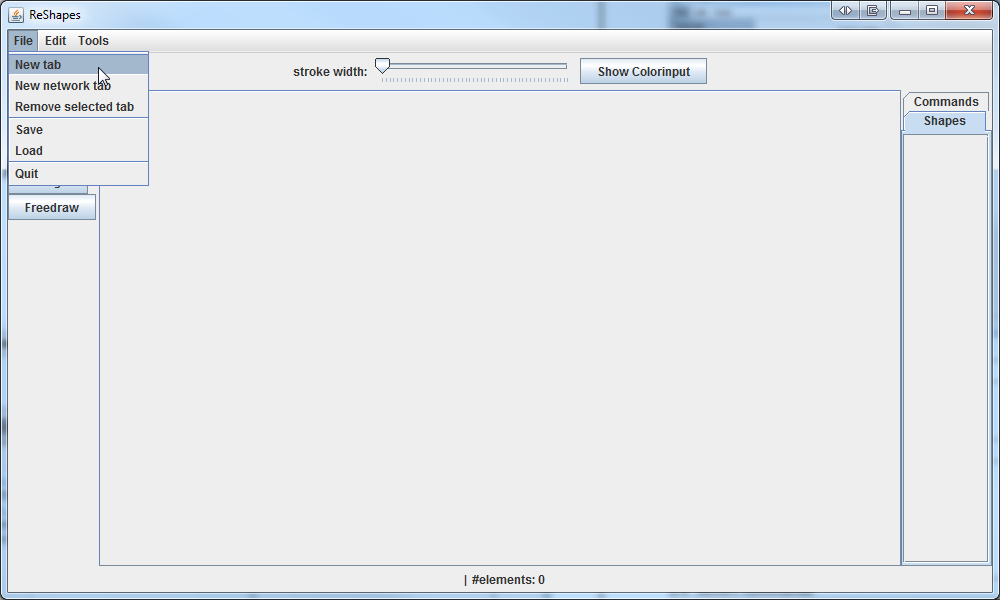
\includegraphics[width=1\textwidth]{img/add_new_tab_1} \\
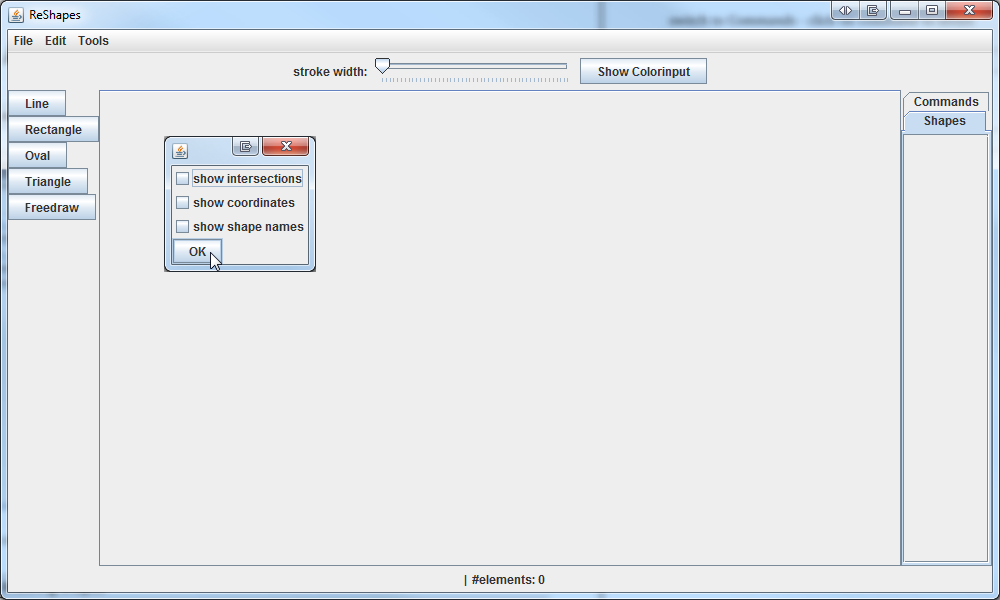
\includegraphics[width=1\textwidth]{img/add_new_tab_2} 

The presented options in the dialog modifiy the drawing space:
\begin{itemize}
    \item \textbf{show intersections:} 
        Displays a small red circle on the intersection point of two shapes
    \item \textbf{show coordinates:}
        Draws a coordinate system instead of the plain white background
    \item \textbf{show shape names:}
        Writes the name of each drawn shape besides it
\end{itemize}

After pressing \textbf{OK} a new tab appears. \\
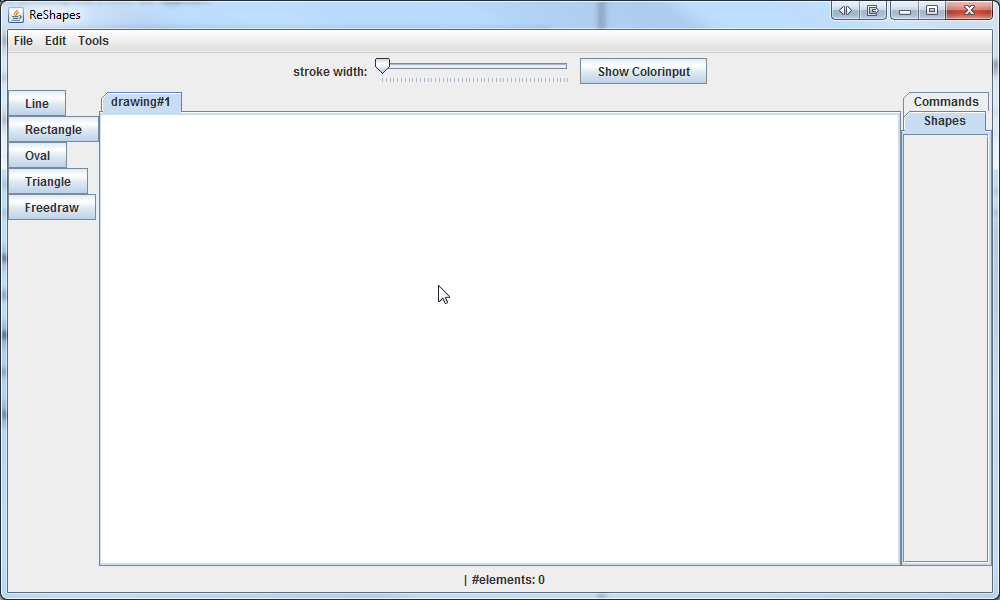
\includegraphics[width=1\textwidth]{img/add_new_tab_3} 

\section{Drawing shapes}

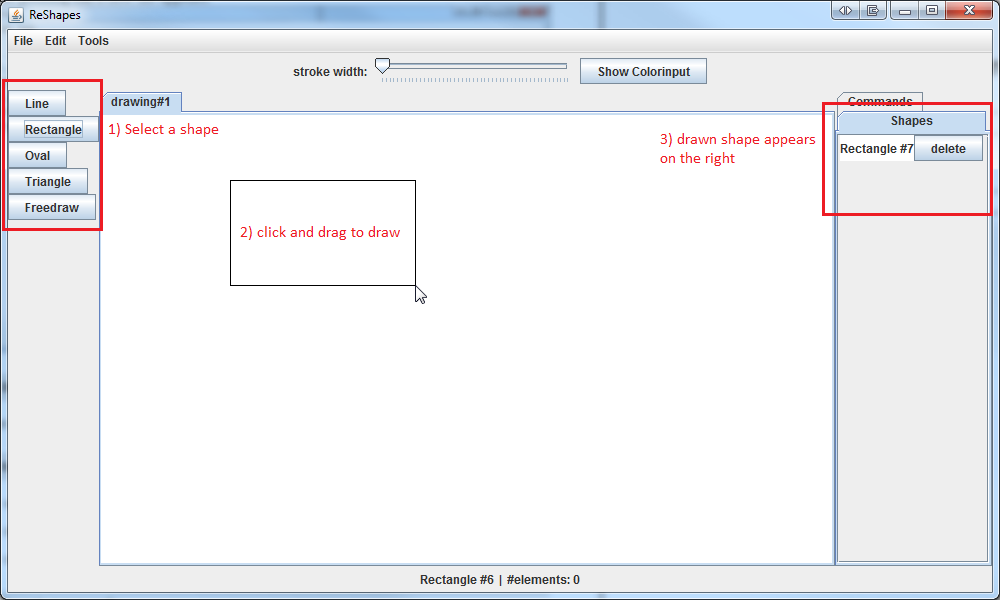
\includegraphics[width=1\textwidth]{img/drawing_shape}

\section{Edit drawn shapes}

\textbf{Set stroke width and color:} \\
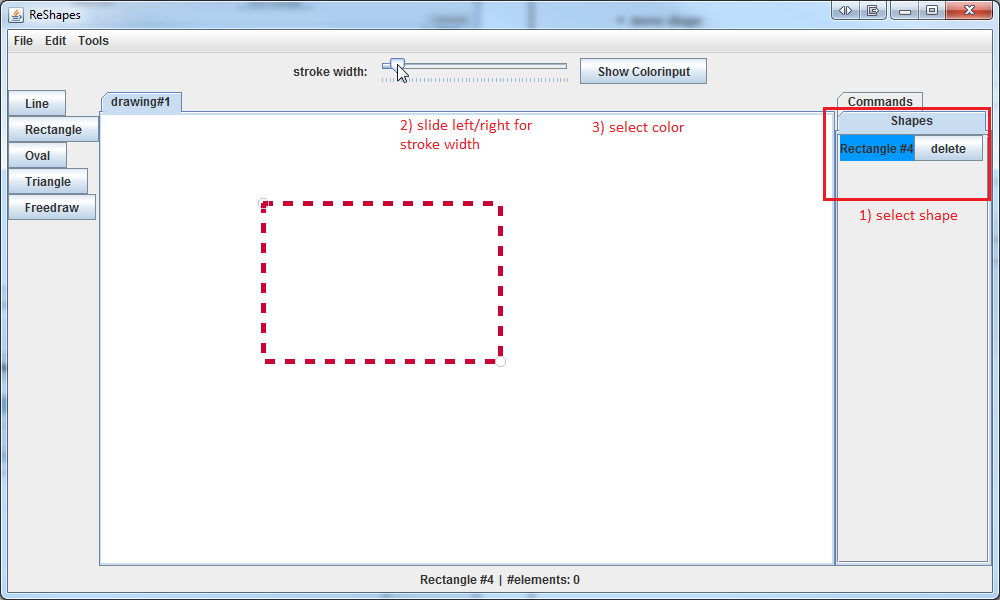
\includegraphics[width=1\textwidth]{img/set_stroke} \\

\textbf{Move shape around:} \\
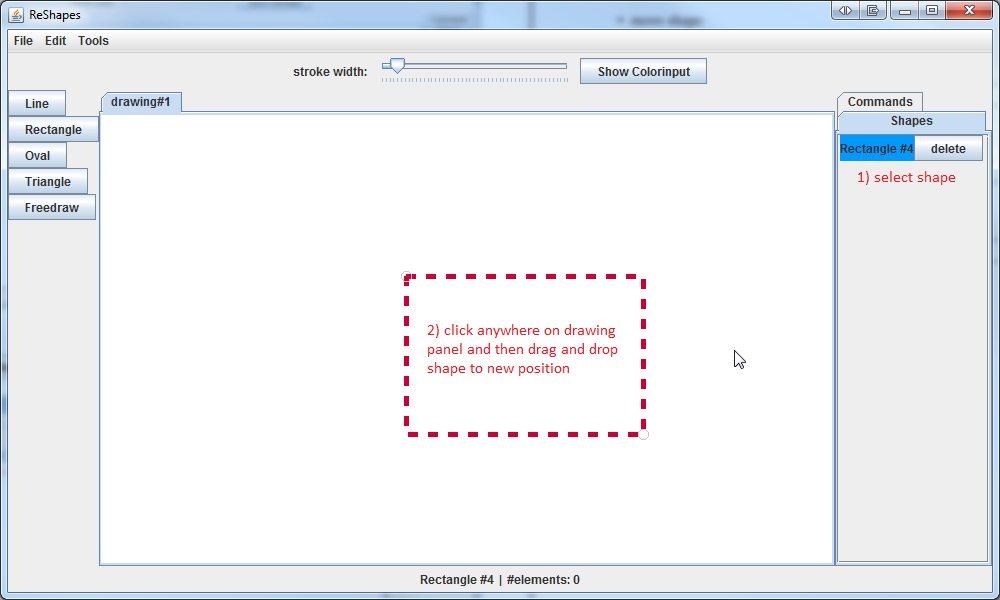
\includegraphics[width=1\textwidth]{img/move_shape} \\

\textbf{Resize shape (not possible with Freedraw):} \\
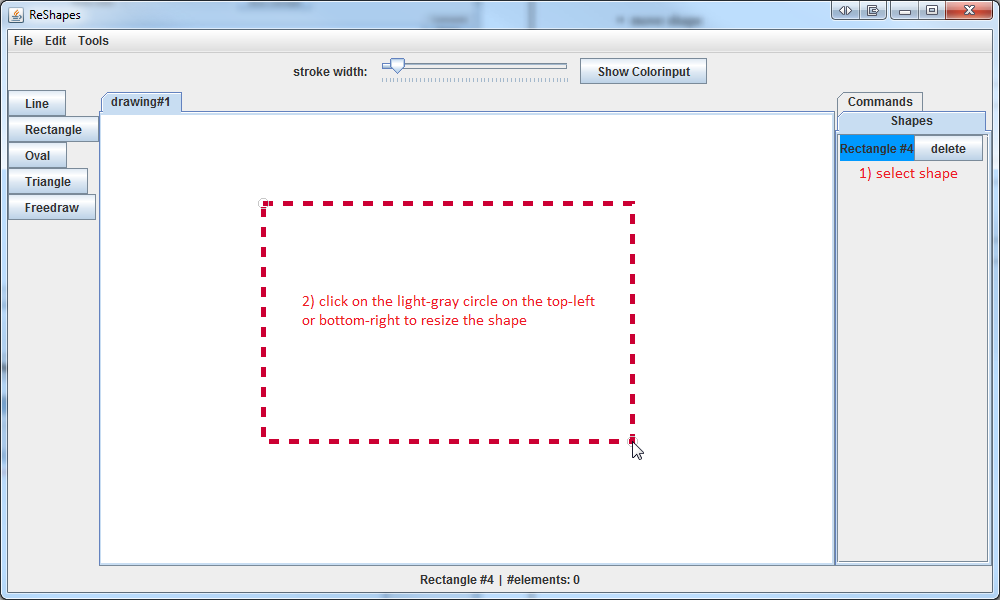
\includegraphics[width=1\textwidth]{img/resize_shape}

\section{Merge tabs}

When merging tabs all drawn shapes of the target tab are copied to the current tab.

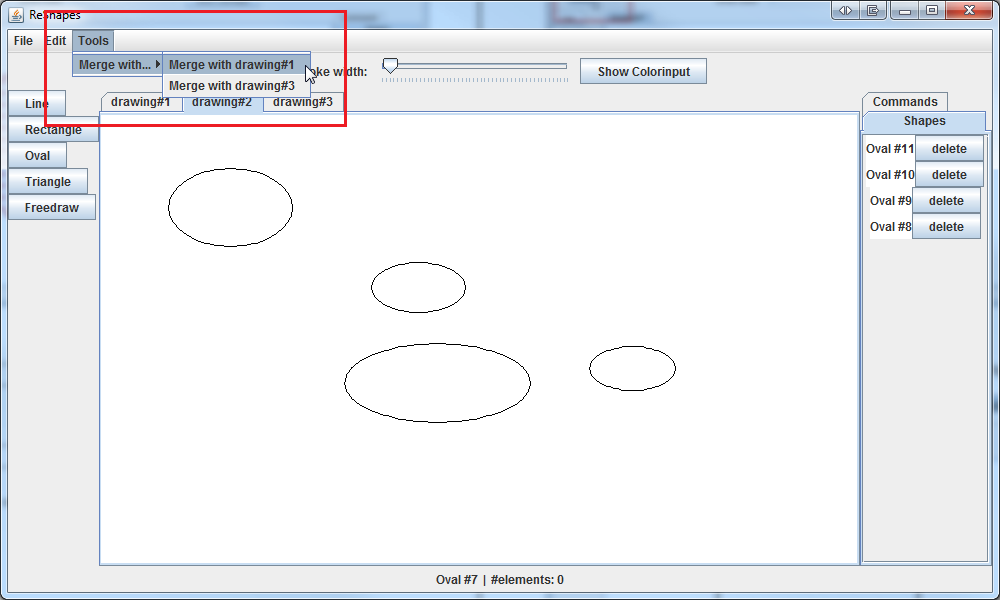
\includegraphics[width=1\textwidth]{img/merge_tabs}

\section{Undo actions}

It is possible to undo following actions:
\begin{itemize}
    \item Delete shape
    \item Create shape
    \item Edit shape
    \item Merging of tabs
\end{itemize}

On way to undo actions is to use the menu \textbf{Edit $\rightarrow$ Undo}: \\
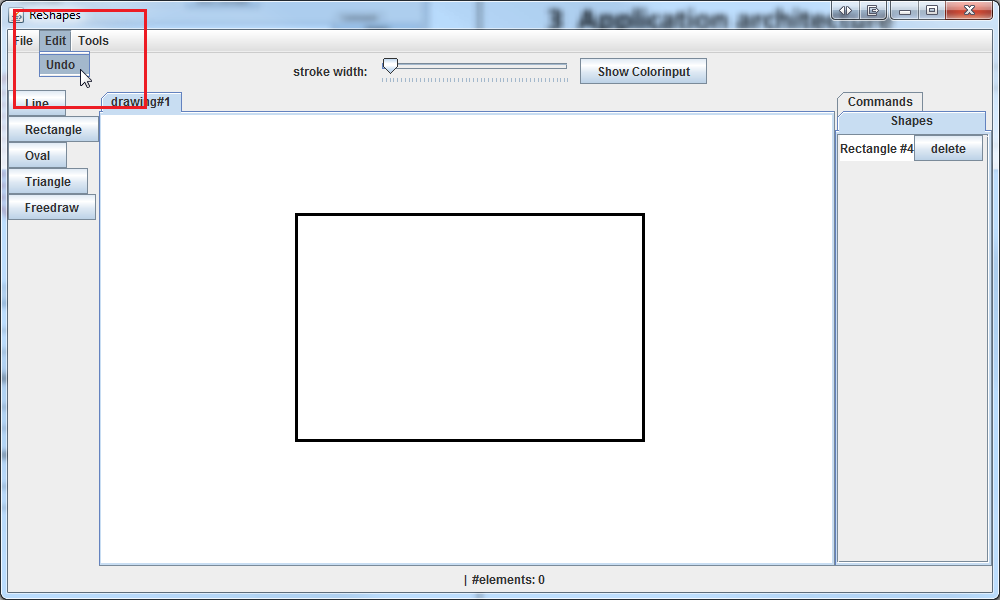
\includegraphics[width=1\textwidth]{img/undo_action_1} \\

The other way to undo actions is to use the \textbf{Commands} panel on the right side and click on the actions you want to undo: \\
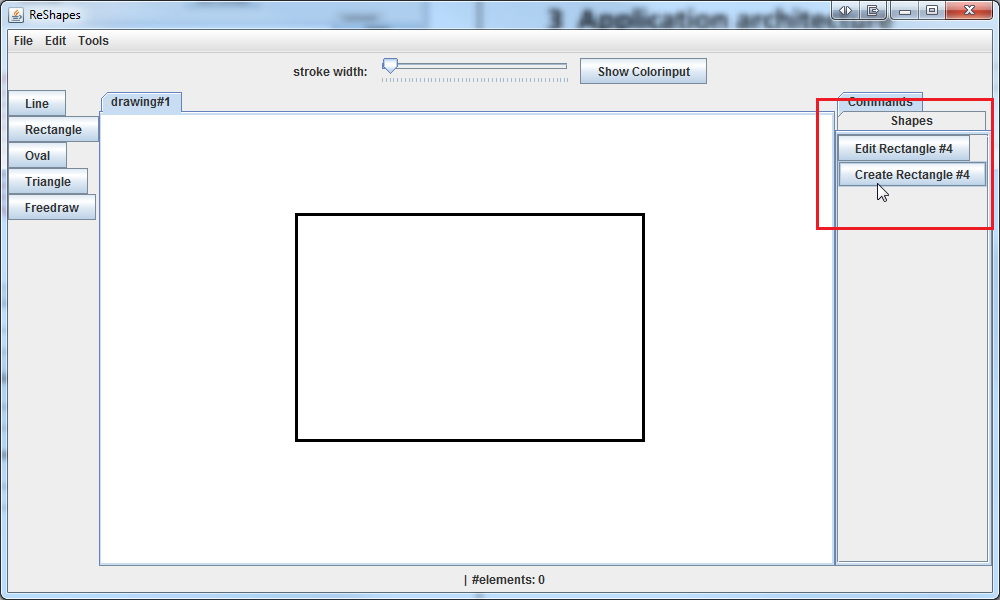
\includegraphics[width=1\textwidth]{img/undo_action_2}

\section{Save and Load}

You can save and load the currently selected tab with \textbf{File $\rightarrow$ Save/Load}: \\
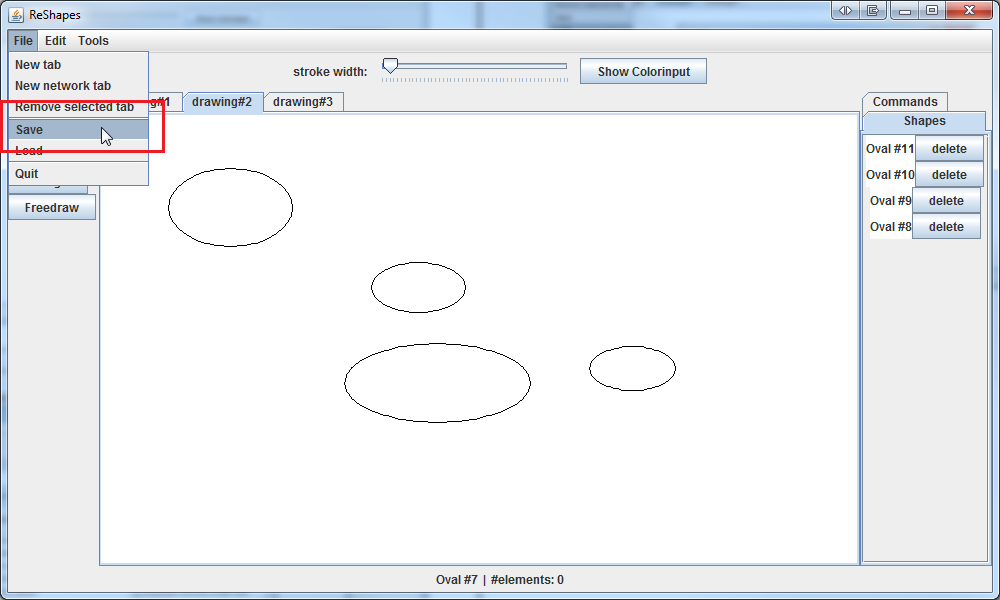
\includegraphics[width=1\textwidth]{img/save} \\
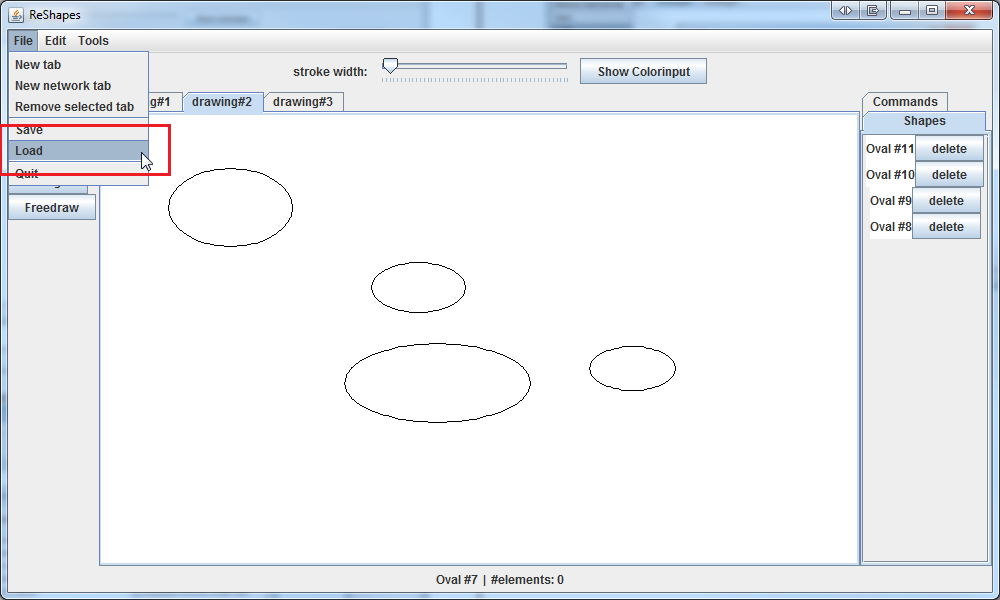
\includegraphics[width=1\textwidth]{img/load} \\

\section{Network tab}

Besides drawing locally it is possible to draw with two or more people onto the same drawing pane over network.
The first step to do so is to start \textit{reshapes.network.ReshapesServer} with two command line arguments. 
Both arguments specifiy the port the server listens to for new clients and updates. \\
After the server is started the client can connect to the server with \textbf{File $\rightarrow$ New network tab}: \\
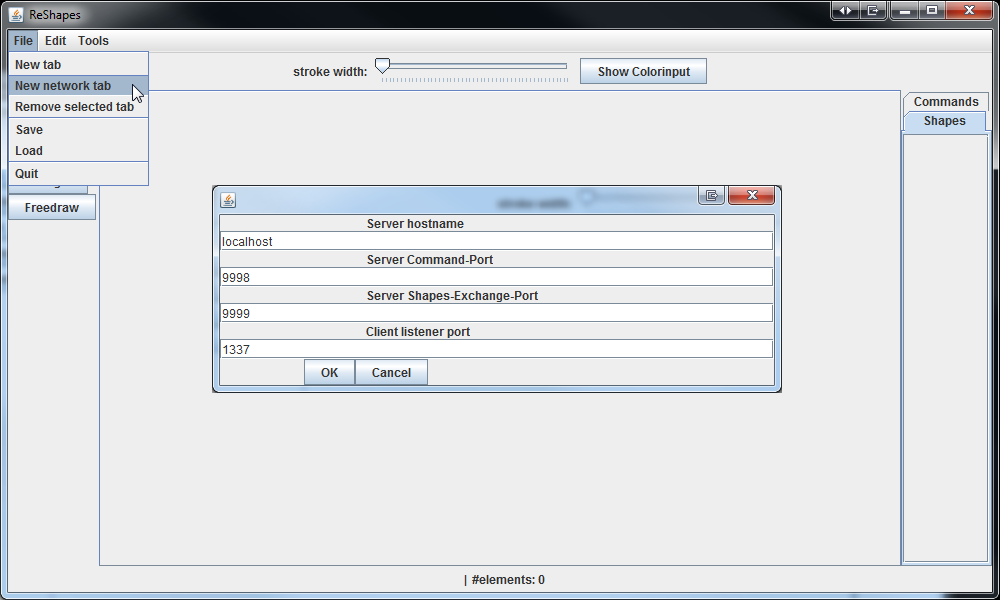
\includegraphics[width=1\textwidth]{img/new_network_tab}

The first three fields defines the hostname and ports of the server and the field \textbf{Client listener port} specifies the port to which the server sends updates.
